\chapter{Resultados}
\label{chap:result}
Os resultados obtidos nos desafios foram:
%--------- NEW SECTION ----------------------
\section{Webots}

Cada um dos 16 sensores de distância incluídos no Pionner são encontrados no arquivo de controle do robô challengecontroller.c
e contêm valores de peso para cada roda, que são baseados na posição do sensor no robô e mostram como sua leitura influencia o 
comportamento do duas rodas. Além disso, o valor do peso auxilia na tomada de decisão, pois, se a leitura de algum sensor cair 
abaixo do valor mínimo definido, significa que o robô está próximo a um obstáculo e deve mudar de direção usando um dos casos acima. 
No final, ele foi usado para determinar o comportamento do robô em todos os valores de peso em cada roda vezes um fator de velocidade, 
que é dependente tanto da relação de leitura do sensor quanto do valor de distância mínima.

Também faz parte do controle o sensor de luz que foi adicionado para completar o desafio, 
este sensor ativa o estado STOP quando detecta um brilho maior que 750 W / m2 e assim o desafio é concluído.

As fotos mostram o pioneer iniciando, chegando na área luminosa e parando no tempo correto, completando assim o desafio proposto,
para uma melhor visualização da solução tem um link do video logo abaixo e o controle pode ser encontrado no repositório https://github.com/marcellabecker/desafiorobotica 

\begin{figure} [h!]	
    \centering
    \caption{Pioneer iniciando o percurso}
    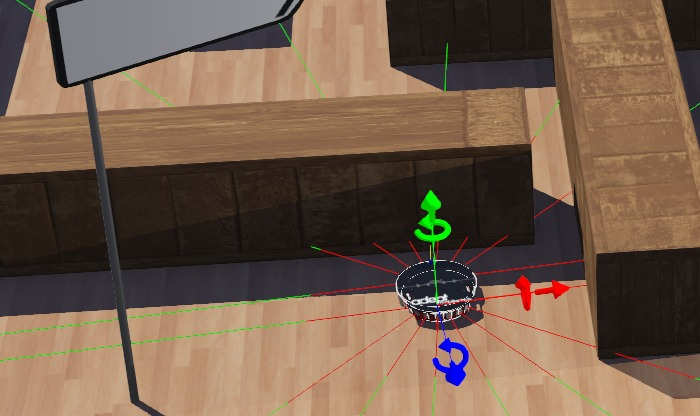
\includegraphics[width=0.5\textwidth]{inicio.jpeg}
    \caption*{Fonte:Própria.}
    \label{fig:inciodopercurso}
\end{figure}

\begin{figure} [h!]	
    \centering
    \caption{Pioneer completando o percurso}
    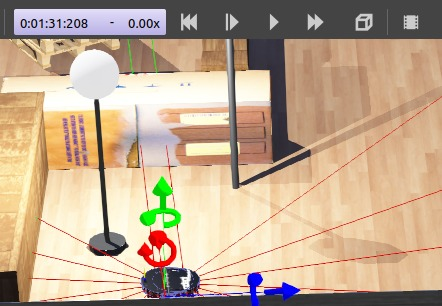
\includegraphics[width=0.4\textwidth]{fim.jpeg}
    \caption*{Fonte:Própria.}
    \label{fig:fimdopercurso}
\end{figure}



Link para assistir ao vídeo:https://www.youtube.com/watch?v=RftRevxZUOE


\label{sec:testu}
\lipsum[1]

\section{Integração do sistema}
\label{sec:intsis}
\lipsum[1]

%--------- NEW SECTION ----------------------
\section{Testes integrados}
\label{sec:testi}
\lipsum[1]







